\documentclass[10pt,a4paper]{article}
\usepackage[T1]{fontenc}
\usepackage[utf8]{inputenc}
\usepackage[brazil]{babel}
\usepackage{lmodern}
\usepackage{amsmath,amssymb,bm}
\usepackage{graphicx}
\usepackage{booktabs}
\usepackage{array}
\usepackage{float}
\usepackage{microtype}
\usepackage{caption}
\usepackage{geometry}
\usepackage{fancyhdr}
\usepackage{hyperref}
\geometry{left=2.25cm,right=2.15cm,top=1.95cm,bottom=1.80cm}
\hypersetup{colorlinks=false,pdfauthor={Rafael Costa Coutinho},pdftitle={Análise dinâmica e representação em espaço de estados de um campo de produção de petróleo operado por BCS}}
\captionsetup{font=small,labelfont=bf,skip=4pt}
\setlength{\parindent}{1.2em}
\setlength{\parskip}{2pt}
\setlength{\textfloatsep}{8pt plus 2pt minus 2pt}
\setlength{\floatsep}{8pt plus 2pt minus 2pt}
\setlength{\intextsep}{7pt plus 2pt minus 2pt}
\renewcommand{\arraystretch}{1.13}
\pagestyle{fancy}
\fancyhf{}
\fancyhead[L]{\footnotesize Análise dinâmica de um campo de produção operado por BCS}
\fancyhead[R]{\footnotesize UFBA}
\fancyfoot[C]{\thepage}
\renewcommand{\headrulewidth}{0.3pt}
\newcommand{\mat}[1]{\mathbf{#1}}
\newcommand{\bcs}{\mathrm{BCS}}
\newcommand{\fbhp}{\mathrm{FBHP}}
\newcommand{\man}{\mathrm{man}}
\newcommand{\tr}{\mathrm{tr}}
\newcommand{\zoh}{\mathrm{ZOH}}
\newcommand{\xhat}{\hat{\mat{x}}}
\newcommand{\uhat}{\hat{\mat{u}}}
\newcommand{\zhat}{\hat{\mat{z}}}
\newcommand{\yhat}{\hat{\mat{y}}}
\begin{document}
\begin{center}
{\Large\bfseries Análise dinâmica e representação em espaço de estados de um campo de produção de petróleo operado por BCS\par}
\vspace{4pt}
{\normalsize Rafael Costa Coutinho e Guilherme Rocha}\par
{\small Universidade Federal da Bahia --- Engenharia de Controle e Automação Industrial}\par
\vspace{5pt}
\end{center}

\noindent\textbf{Resumo.} Este trabalho apresenta a análise dinâmica de um campo de produção de petróleo composto por dois poços equipados com Bombeio Centrífugo Submerso (BCS), interligados a um \textit{manifold} e a uma bomba \textit{booster}. A partir da representação fenomenológica por equações diferenciais-algébricas, foram investigadas as respostas do sistema a perturbações operacionais, a linearização em torno de um ponto estacionário, a estabilidade local, as formas canônicas e a discretização do modelo linearizado. Os resultados permitiram caracterizar a interação entre os poços, identificar modos dinâmicos com diferentes escalas de tempo e comparar representações contínuas e discretas do processo.\par
\noindent\textbf{Palavras-chave:} Bombeio Centrífugo Submerso; modelo fenomenológico; espaço de estados; estabilidade; discretização.

\section{Introdução}
O Bombeio Centrífugo Submerso (BCS) está entre os métodos de elevação artificial mais utilizados na produção de petróleo, destacando-se por sua capacidade de operar em grandes profundidades e fornecer elevadas vazões. Sua aplicação torna-se especialmente relevante quando a energia natural do reservatório não é suficiente para assegurar as condições de produção desejadas. Entretanto, a operação de sistemas com BCS está sujeita a limitações hidráulicas e operacionais, associadas às pressões, às vazões e às características de funcionamento das bombas.

Nesse contexto, a utilização de modelos matemáticos permite investigar o comportamento do processo em diferentes condições de operação sem a necessidade de realizar perturbações diretamente no campo. Para sistemas com múltiplos poços conectados a uma estrutura de produção comum, essa análise é particularmente importante, uma vez que alterações em um dos poços podem afetar as condições de operação dos demais. A representação em espaço de estados permite descrever simultaneamente a dinâmica das variáveis internas e suas relações com as entradas manipuladas, constituindo uma ferramenta adequada à análise de sistemas multivariáveis.

Este trabalho analisa o comportamento dinâmico de uma adaptação do modelo fenomenológico apresentado por Rønning~\cite{ronning2011}, considerando um campo formado por dois poços operados por BCS. Inicialmente, são avaliadas as respostas do sistema não linear a perturbações nas entradas operacionais. Em seguida, o modelo é linearizado em torno de uma condição estacionária, permitindo investigar a estabilidade, obter representações nas formas canônicas controlável, observável e de Jordan e comparar métodos de discretização. A análise busca caracterizar o processo e verificar a capacidade do modelo linear de reproduzir seu comportamento nas proximidades do ponto de operação.

\section{Campo de produção de petróleo}
O sistema estudado consiste em uma adaptação do modelo proposto por Rønning~\cite{ronning2011}, considerando dois poços de produção equipados com BCS e conectados a um \textit{manifold} comum. Cada poço possui uma válvula \textit{choke}, responsável pela regulação da vazão produzida, enquanto uma bomba \textit{booster}, situada a jusante do \textit{manifold}, auxilia no transporte do fluido até as instalações de superfície. A interação entre os poços ocorre por meio da pressão do \textit{manifold}, que depende das vazões recebidas e da vazão encaminhada à linha de transporte.

O modelo fenomenológico é descrito por um sistema de equações
diferenciais-algébricas (DAE). Para a configuração considerada neste
trabalho, com dois poços, o modelo é composto por 8 equações diferenciais
ordinárias e 4 equações algébricas. Para cada poço, com
$i \in \{1,2\}$, são consideradas a pressão de fundo
($p_{\text{FBHP}_i}$), a pressão na entrada da válvula choke
($p^{\text{in}}_{c,i}$), a vazão volumétrica média ($q_i$), a pressão de
entrada da BCS ($p^{\text{in}}_{\text{BCS}_i}$) e o incremento de pressão
gerado pela bomba ($\Delta p_{\text{BCS}_i}$). Para o manifold e a linha
de transporte são consideradas a pressão do manifold ($p_{\text{man}}$)
e a vazão volumétrica de transporte ($q_{\text{tr}}$).

\vspace{-0.5cm}
\begin{figure}[H]
    \centering 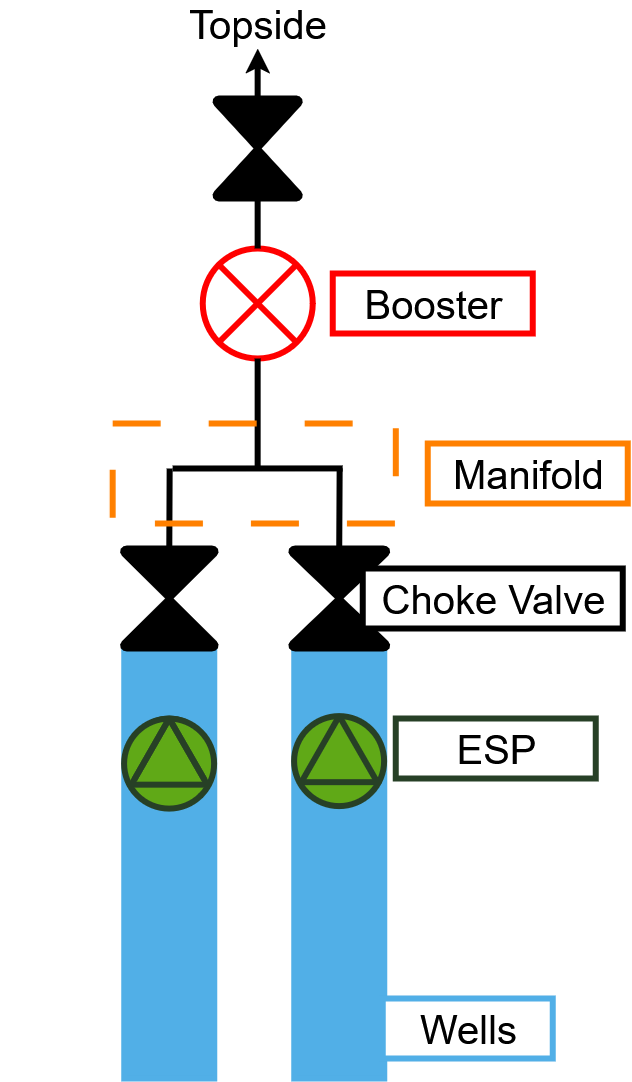
\includegraphics[width=0.20\textwidth]{figuras/20226.2model.drawio.png}
    \caption{Fluxograma do Campo de Produção de Petróleo.}
    \label{fig:validacao_pman}
\end{figure}

Assim, o vetor de estados possui oito componentes, sendo três associados
a cada poço e dois associados ao sistema comum de produção, enquanto o
vetor de variáveis algébricas possui quatro componentes. O conjunto de
equações que descreve a dinâmica do sistema, adaptado de Rønning~\cite{ronning2011}, é dado por:
\begin{align}
\dot{p}_{\text{FBHP}_i} &= \frac{\beta_1}{V_1} \left( PI(p_{r,i} - p_{\text{FBHP}_i}) - q_i \right), \\
\dot{p}^{in}_{c,i} &= \frac{\beta_2}{V_2} \left( q_i - k_{Gc}(z_{c,i}) \sqrt{p^{in}_{c,i} - p_{\text{man}}} \right), \\
\dot{p}_{\text{man}} &= \frac{\beta_{\text{man}}}{V_{\text{man}}} (q_{in,man} - q_{\text{tr}}), \\
\dot{q}_{tr} &= \frac{A_{tr}}{\rho_{tr} l_{tr}} (p_{\text{man}} + \Delta p_{\text{BCS}_i} - p_{\text{topo}}) 
- \frac{(B_0^{tr} + B_1^{tr})}{A_{tr}} \frac{\rho_{tr} q_{\text{tr}}^2}{2}, \\
\dot{q}_i &= \frac{A}{\rho_l} \Bigg( p_{\text{FBHP}_i} - p^{in}_{c,i} + \Delta p_{\text{BCS}_i} +
- \frac{(B_0^1 + B_1^1)}{A_1} \frac{\rho_1 q_i^2}{2}
- \frac{(B_0^2 + B_1^2)}{A_2} \frac{\rho_1 q_i^2}{2} + ... \nonumber \\
-& \rho_1 g (h_r - h_p) - \rho_2 g (h_r - h_p) \Bigg),\\
p^{in}_{\text{BCS}_i} &= p^{in}_{c,i} + \frac{(B_0^2 + B_1^2)}{2} + 
 \rho_2 q_i^2 + \rho_2 g (h_{p,i} - h_{c,i}) - \Delta p_{\text{BCS}_i}, \\
\Delta p_{\text{BCS}_i} &= \rho_{\text{man}} g H_{BP,i}(f_{BP,i}).
\end{align}

Na qual $\mat{x}\in\mathbb{R}^{8}$ representa os estados diferenciais, $\mat{z}\in\mathbb{R}^{4}$ reúne as variáveis algébricas e $\mat{u}\in\mathbb{R}^{6}$ corresponde às entradas do processo. Esses vetores são definidos por
\begin{align}
\mat{x}&=\begin{bmatrix}p_{\man}&q_{\tr}&p_{\fbhp,1}&p_{c,1}&\bar q_1&p_{\fbhp,2}&p_{c,2}&\bar q_2\end{bmatrix}^{T},\nonumber\\
\mat{z}&=\begin{bmatrix}p_{\mathrm{intake},1}&\Delta p_{\bcs,1}&p_{\mathrm{intake},2}&\Delta p_{\bcs,2}\end{bmatrix}^{T},\nonumber\\
\mat{u}&=\begin{bmatrix}f_{\mathrm{BP}}&p_{\mathrm{topside}}&f_{\bcs,1}&\alpha_1&f_{\bcs,2}&\alpha_2\end{bmatrix}^{T},\label{eq:vetores}
\end{align}
sendo $f_{\mathrm{BP}}$ a frequência da bomba \textit{booster}, $f_{\bcs,i}$ a frequência de operação da BCS de cada poço, $\alpha_i$ a abertura da respectiva válvula \textit{choke} e $p_{\mathrm{topside}}$ a pressão na saída da linha de transporte.

\subsection{Ponto de operação e resposta dinâmica}
Para a determinação do ponto estacionário, foram fixadas as frequências da bomba \textit{booster} e das BCS em $45$ Hz e $50$ Hz, respectivamente, as aberturas das válvulas em $0{,}8$ e a pressão de saída em $1$ bar. A condição de equilíbrio foi obtida numericamente impondo-se as condições estacionárias
$f(x_{ss},z_{ss},u_{ss})=0$ e
$g(x_{ss},z_{ss},u_{ss})=0$. Os valores resultantes encontram-se na Tabela~\ref{tab:ss}.

\begin{table}[htbp]\centering\small
\caption{Ponto de operação estacionário do campo com dois poços.}\label{tab:ss}
\begin{tabular}{@{}llrlr@{}}\toprule
Vetor & Variável & Valor & Variável & Valor\\\midrule
$\mat{x}_{ss}$ & $p_{\man}/\mathrm{bar}$ & 66,9278 & $q_{\tr}/(\mathrm{m}^3/\mathrm{h})$ & 175,9557\\
& $p_{\fbhp,1}/\mathrm{bar}$ & 224,3109 & $p_{c,1}/ \mathrm{bar}$ & 143,9351\\
& $\bar q_1/(\mathrm{m}^3/\mathrm{h})$ & 90,4961 & $p_{\fbhp,2}/ \mathrm{bar}$ & 205,0449\\
& $p_{c,2}/\mathrm{bar}$ & 135,6019 & $\bar q_2/(\mathrm{m}^3/ \mathrm{h})$ & 85,4595\\\midrule
$\mat{z}_{ss}$ & $p_{\mathrm{intake},1}/\mathrm{bar}$ & 189,8151 & $\Delta p_{\bcs,1}/ \mathrm{bar}$ & 76,7618\\
& $p_{\mathrm{intake},2}/\mathrm{bar}$ & 168,6196 & $\Delta p_{\bcs,2}/ \mathrm{bar}$ & 82,5215\\\bottomrule
\end{tabular}
\end{table}

A partir dessa condição, foram aplicadas perturbações individuais nas cinco entradas manipuladas, mantendo $p_{\mathrm{topside}}$ constante. As alterações consistiram em pulsos de $2$ Hz nas frequências ou de $0{,}03$ nas aberturas das válvulas, seguidos do retorno aos respectivos valores nominais. O horizonte de simulação permitiu observar tanto a resposta transitória quanto a recuperação do equilíbrio após a retirada das perturbações. As Figuras~\ref{fig:input} e~\ref{fig:nl} apresentam, como exemplo, as trajetórias obtidas para uma variação na frequência da BCS do primeiro poço.

\begin{figure}[htbp]\centering
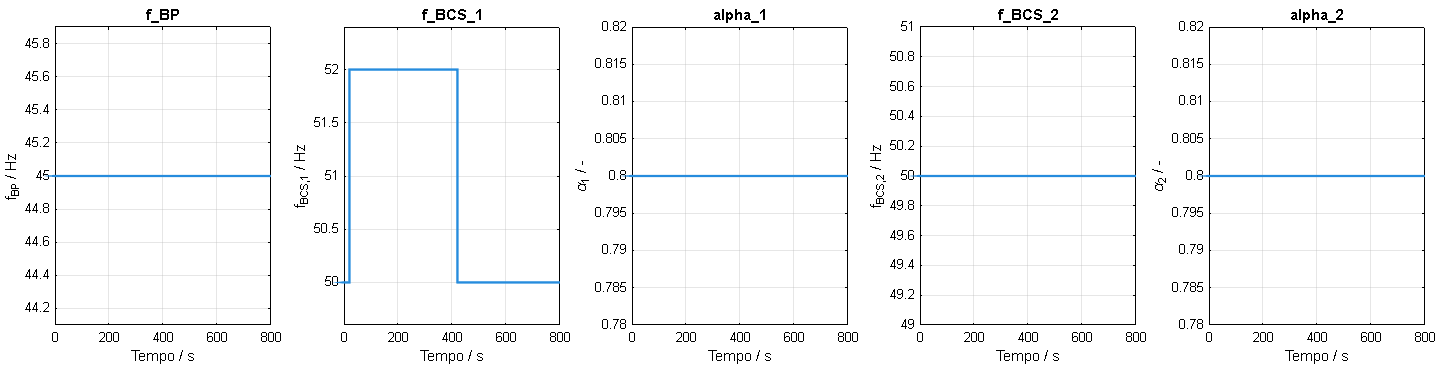
\includegraphics[width=.96\linewidth]{figuras/sistema_entradas.png}
\caption{Perturbação aplicada na frequência da BCS do poço 1, com as demais entradas mantidas em seus valores nominais. Fonte: elaboração própria.}\label{fig:input}
\end{figure}
\begin{figure}[htbp]\centering
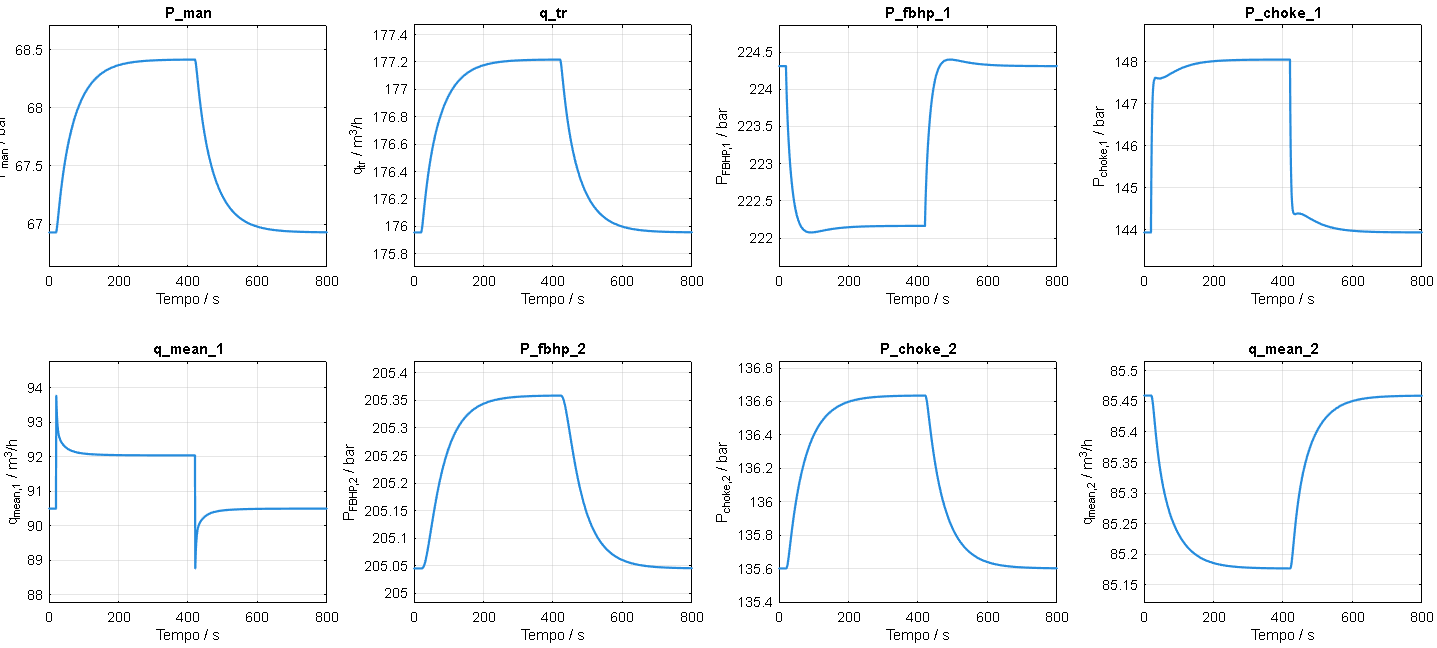
\includegraphics[width=.98\linewidth]{figuras/sistema_saidas.png}
\caption{Respostas dos oito estados do modelo não linear à perturbação na frequência da BCS do poço 1. Fonte: elaboração própria.}\label{fig:nl}
\end{figure}
Observa-se que a alteração em $f_{\bcs,1}$ influencia diretamente as condições de produção do primeiro poço, mas também modifica a pressão do \textit{manifold}, a vazão total de transporte e as variáveis associadas ao segundo poço. Esse comportamento evidencia o acoplamento hidráulico existente entre os subsistemas. Após a retirada do pulso, as trajetórias retornam gradualmente às condições estacionárias, enquanto as pressões algébricas associadas às bombas acompanham as mudanças de regime, conforme apresentado na Figura~\ref{fig:alg}.
\begin{figure}[htbp]\centering
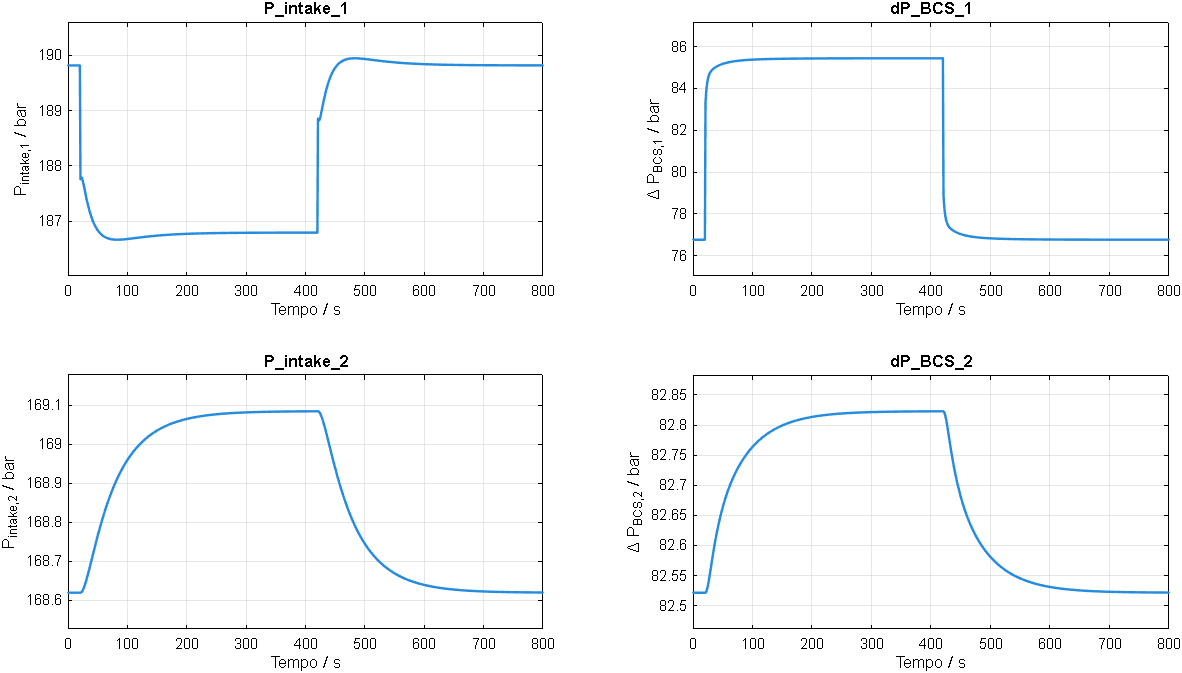
\includegraphics[width=.76\linewidth]{figuras/sistema_algebricas.png}
\caption{Comportamento das pressões de sucção e dos incrementos de pressão das BCS durante a perturbação no poço 1. Fonte: elaboração própria.}\label{fig:alg}
\end{figure}
\section{Linearização do modelo fenomenológico}
A linearização foi realizada em torno da condição estacionária $\bigl(\mat{x}_{ss},\mat{z}_{ss},\mat{u}_{ss}\bigr)$, por meio da expansão de Taylor de primeira ordem das equações diferenciais e algébricas. As variáveis de desvio são representadas pelo símbolo de chapéu, de modo que
\begin{equation}
\xhat=\mat{x}-\mat{x}_{ss},\qquad
\zhat=\mat{z}-\mat{z}_{ss},\qquad
\uhat=\mat{u}-\mat{u}_{ss}.
\label{eq:desvios}
\end{equation}
Nesta análise, os desvios são expressos nas mesmas unidades das variáveis originais. A expansão linear das equações do modelo fornece
\begin{align}
\dot{\xhat}&=\mat{F}_{x}\xhat+\mat{F}_{z}\zhat+\mat{F}_{u}\uhat,\label{eq:lin_dae_a}\\
\mat{0}&=\mat{G}_{x}\xhat+\mat{G}_{z}\zhat+\mat{G}_{u}\uhat,\label{eq:lin_dae_b}
\end{align}
na qual as matrizes $\mat{F}_{x}$, $\mat{F}_{z}$, $\mat{F}_{u}$, $\mat{G}_{x}$, $\mat{G}_{z}$ e $\mat{G}_{u}$ correspondem às respectivas matrizes jacobianas, avaliadas no ponto de equilíbrio.

Admitindo-se $\mat{G}_{z}$ não singular, as variáveis algébricas são eliminadas da representação dinâmica. Dessa forma, obtêm-se
\begin{align}
\zhat&=-\mat{G}_{z}^{-1}\mat{G}_{x}\xhat-\mat{G}_{z}^{-1}\mat{G}_{u}\uhat,\label{eq:elim_alg}\\
\mat{A}&=\mat{F}_{x}-\mat{F}_{z}\mat{G}_{z}^{-1}\mat{G}_{x},\nonumber\\
\mat{B}&=\mat{F}_{u}-\mat{F}_{z}\mat{G}_{z}^{-1}\mat{G}_{u}.\label{eq:matrizes_lin}
\end{align}
O modelo linearizado em espaço de estados é, portanto, representado por
\begin{equation}
\dot{\xhat}=\mat{A}\xhat+\mat{B}\uhat,\qquad
\yhat=\mat{C}\xhat.\label{eq:espaco_estados}
\end{equation}
Foram consideradas as cinco entradas manipuladas e os oito estados diferenciais como saídas do sistema, resultando em $\mat{A}\in\mathbb{R}^{8\times8}$, $\mat{B}\in\mathbb{R}^{8\times5}$ e $\mat{C}=\mat{I}_8$. As quatro variáveis algébricas são obtidas separadamente pela relação apresentada na Equação~\eqref{eq:elim_alg}.

A representatividade do modelo linearizado foi avaliada
por meio da comparação de sua resposta com a do modelo
fenomenológico não linear, considerando perturbações
na frequência da BCS do poço 1 ($f_{\mathrm{BCS},1}$).
Como variável de saída, considerou-se o incremento
de pressão desenvolvido pela bomba
($\Delta p_{\mathrm{BCS},1}$).
Inicialmente, aplicou-se uma pequena perturbação
de 50 para 52 Hz, buscando avaliar a capacidade
do modelo linearizado de representar o comportamento
do sistema nas proximidades do ponto de operação.
Posteriormente, a frequência foi elevada para 65 Hz,
permitindo investigar as diferenças entre os modelos
para uma condição mais distante do equilíbrio.
\begin{figure}[H]\centering
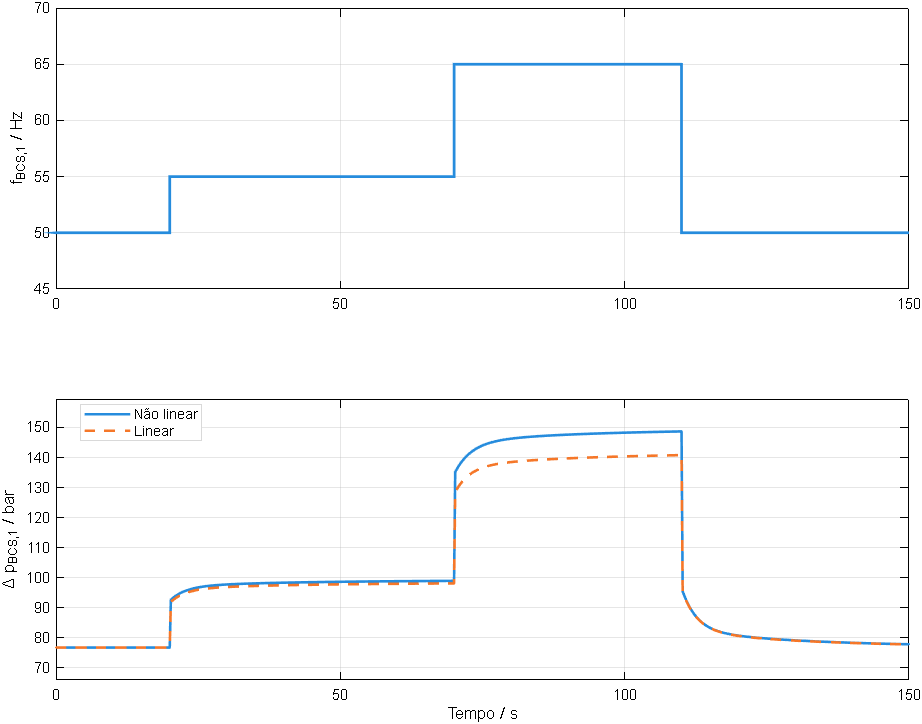
\includegraphics[width=.74\linewidth]{figuras/comparacao.png}
\caption{Comparação entre as respostas dos modelos linearizado e não linear para o incremento de pressão da BCS do poço 1, considerando perturbações na frequência de operação. Fonte: elaboração própria.}\label{fig:comp}
\end{figure}
As trajetórias apresentam comportamento próximo para as perturbações analisadas, com diferenças mais perceptíveis quando a variação da entrada é elevada. O resultado é coerente com a natureza local da linearização, cuja precisão depende da proximidade em relação ao ponto de operação considerado.

\section{Análise de estabilidade}
A estabilidade do modelo linearizado foi investigada a partir dos autovalores da matriz $\mat{A}$. Para um sistema linear contínuo, a condição de estabilidade assintótica é satisfeita quando todos os autovalores apresentam parte real estritamente negativa, isto é, $\operatorname{Re}(\lambda_i)<0$.

\begin{table}[htbp]\centering\small
\caption{Autovalores da matriz dinâmica $\mat{A}$ no ponto de operação.}\label{tab:poles}
\begin{tabular}{@{}rrrr@{}}\toprule
$\lambda_1/\mathrm{s}^{-1}$ & $\lambda_2/\mathrm{s}^{-1}$ & $\lambda_3/\mathrm{s}^{-1}$ & $\lambda_4/\mathrm{s}^{-1}$\\\midrule
$-203{,}1294$ & $-148{,}9941$ & $-2{,}4261$ & $-0{,}4084$\\\midrule
$\lambda_5/\mathrm{s}^{-1}$ & $\lambda_6/\mathrm{s}^{-1}$ & $\lambda_7/\mathrm{s}^{-1}$ & $\lambda_8/\mathrm{s}^{-1}$\\\midrule
$-0{,}3850$ & $-0{,}0676$ & $-0{,}0553$ & $-0{,}0182$\\\bottomrule
\end{tabular}
\end{table}

Conforme apresentado na Tabela~\ref{tab:poles}, todos os autovalores encontram-se no semiplano esquerdo do plano complexo. Portanto, o sistema linearizado é assintoticamente estável, indicando estabilidade local do ponto de equilíbrio do modelo não linear, sob as hipóteses usuais de regularidade da linearização. A diferença entre os módulos dos autovalores evidencia a coexistência de modos rápidos e lentos, associados a diferentes escalas de tempo do processo.

Para complementar essa análise, foram consideradas 12 condições iniciais próximas ao equilíbrio, com variações limitadas a $\pm5\%$ dos valores estacionários dos estados. As trajetórias foram determinadas a partir da evolução do sistema linear homogêneo, dada por $\xhat(t)=e^{\mat{A}t}\xhat(0)$, e representadas em três projeções tridimensionais do espaço de estados.
\begin{figure}[htbp]\centering
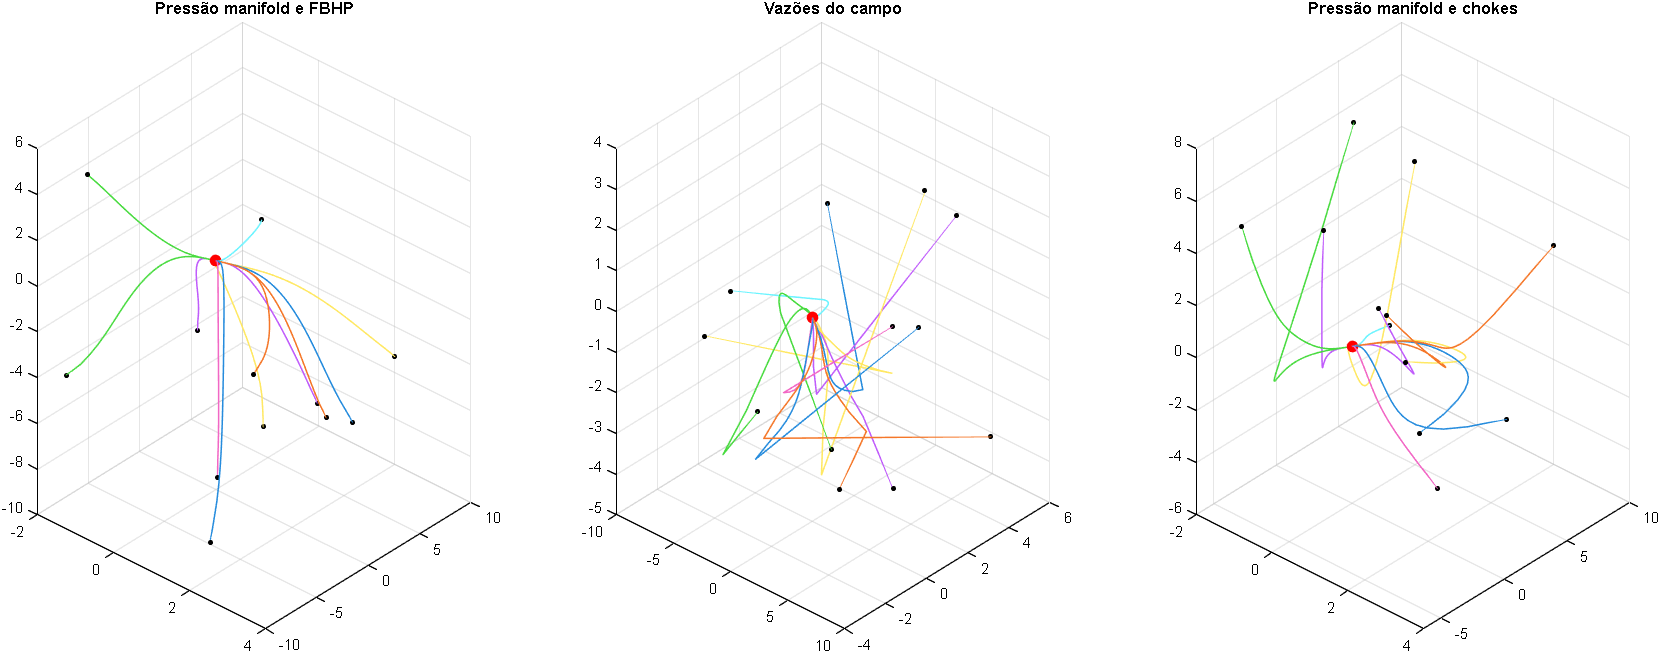
\includegraphics[width=.98\linewidth]{figuras/estabilidade.png}
\caption{Projeções do espaço de estados para diferentes condições iniciais próximas ao equilíbrio. A origem representa a condição de desvio nulo. Fonte: elaboração própria.}\label{fig:estab}
\end{figure}

Na Figura~\ref{fig:estab}, as trajetórias convergem para a origem, em concordância com a distribuição dos autovalores. Esse comportamento confirma a estabilidade assintótica do modelo linearizado, sem constituir uma demonstração de estabilidade global para o sistema não linear.

\section{Formas canônicas}
A partir da representação linear em espaço de estados, obteve-se a matriz de funções de transferência por meio de
\begin{equation}
\mat{G}(s)=\mat{C}(s\mat{I}-\mat{A})^{-1}\mat{B}.\label{eq:tf}
\end{equation}
Como o sistema possui oito saídas e cinco entradas manipuladas, a matriz $\mat{G}(s)$ apresenta dimensão $8\times5$, totalizando 40 relações entre entradas e saídas. Para a análise das formas canônicas, foi selecionada a relação entre a frequência da BCS do poço 1 e sua vazão média, definida por $G(s)=\bar Q_1(s)/F_{\bcs,1}(s)$. Após a realização das reduções por cancelamento de polos e zeros comuns, com tolerância numérica de $10^{-5}$, obteve-se uma realização de sexta ordem.


\subsection{Forma canônica controlável}

A realização na forma canônica controlável, correspondente à função de transferência selecionada, resultou na seguinte matriz de estados:

\begingroup
\small
\setlength{\arraycolsep}{3pt}
\begin{equation}
\mat{A}_{c}\approx
\begin{bmatrix}
-204{,}0638 & -190{,}0854 & -55{,}9060 & -5{,}4805 & -0{,}20156 & -0{,}002169\\
1 & 0 & 0 & 0 & 0 & 0\\
0 & 1 & 0 & 0 & 0 & 0\\
0 & 0 & 1 & 0 & 0 & 0\\
0 & 0 & 0 & 1 & 0 & 0\\
0 & 0 & 0 & 0 & 1 & 0
\end{bmatrix}.
\label{eq:Ac}
\end{equation}
\endgroup

O vetor de entrada e a matriz de saída dessa realização são dados, aproximadamente, por

\begingroup
\small
\setlength{\arraycolsep}{3pt}
\begin{equation}
\begin{aligned}
\mat{B}_{c} &=
\begin{bmatrix}
1 & 0 & 0 & 0 & 0 & 0
\end{bmatrix}^{T},\\[6pt]
\mat{C}_{c} &\approx
\begin{bmatrix}
385{,}2165 & 297{,}6027 & 70{,}6511 &
5{,}8657 & 0{,}182525 & 0{,}001676
\end{bmatrix}.
\end{aligned}
\end{equation}
\endgroup

A estrutura de $\mat{A}_{c}$ concentra os coeficientes do polinômio característico na primeira linha e apresenta elementos unitários na subdiagonal.

\subsection{Forma canônica observável}

A forma canônica observável foi obtida por dualidade em relação à realização controlável. Assim, a matriz de estados assumiu a seguinte configuração:

\begingroup
\small
\setlength{\arraycolsep}{3pt}
\begin{equation}
\mat{A}_{o}=\mat{A}_{c}^{T}\approx
\begin{bmatrix}
-204{,}0638 & 1 & 0 & 0 & 0 & 0\\
-190{,}0854 & 0 & 1 & 0 & 0 & 0\\
-55{,}9060 & 0 & 0 & 1 & 0 & 0\\
-5{,}4805 & 0 & 0 & 0 & 1 & 0\\
-0{,}20156 & 0 & 0 & 0 & 0 & 1\\
-0{,}002169 & 0 & 0 & 0 & 0 & 0
\end{bmatrix}.
\label{eq:Ao}
\end{equation}
\endgroup

Os demais elementos dessa representação satisfazem $\mat{B}_{o}=\mat{C}_{c}^{T}$ e $\mat{C}_{o}=\mat{B}_{c}^{T}$. Embora os estados internos apresentem uma organização diferente, essa realização mantém a mesma relação entrada--saída do sistema controlável.

\subsection{Forma de Jordan}

Para a obtenção da representação de Jordan, realizou-se uma transformação de similaridade utilizando os autovetores da matriz de estados da realização controlável. Como os autovalores da realização reduzida são distintos e a matriz de autovetores admite inversa, a matriz dinâmica pôde ser representada de forma diagonal, aproximadamente, por

\begingroup
\small
\setlength{\arraycolsep}{3pt}
\begin{equation}
\mat{A}_{J}\approx
\begin{bmatrix}
-203{,}1294 & 0 & 0 & 0 & 0 & 0\\
0 & -0{,}4084 & 0 & 0 & 0 & 0\\
0 & 0 & -0{,}3850 & 0 & 0 & 0\\
0 & 0 & 0 & -0{,}06755 & 0 & 0\\
0 & 0 & 0 & 0 & -0{,}05526 & 0\\
0 & 0 & 0 & 0 & 0 & -0{,}01819
\end{bmatrix}.
\label{eq:Aj}
\end{equation}
\endgroup

Denotando por $\mat{V}$ a matriz formada pelos autovetores, a transformação foi dada por $\mat{A}_{J}=\mat{V}^{-1}\mat{A}_{c}\mat{V}$, $\mat{B}_{J}=\mat{V}^{-1}\mat{B}_{c}$, $\mat{C}_{J}=\mat{C}_{c}\mat{V}$. A estrutura diagonal permite identificar diretamente os modos dinâmicos associados aos autovalores da realização reduzida.

As três realizações foram submetidas a uma mesma entrada em degrau unitário. A Figura~\ref{fig:canon} apresenta os comportamentos dos estados transformados e das saídas correspondentes.

\begin{figure}[H]
\centering
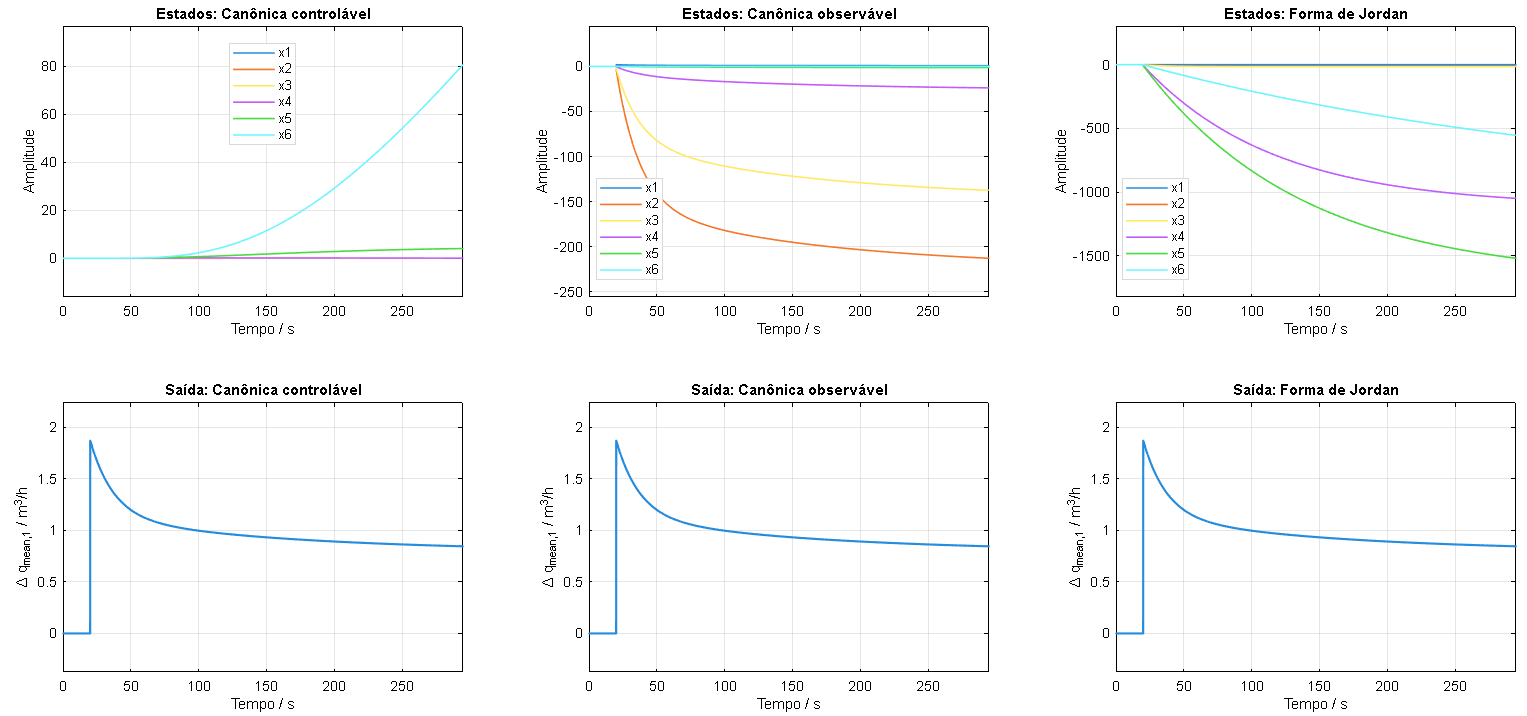
\includegraphics[width=1\linewidth]{figuras/canonicas.png}
\caption{Respostas dos estados e da saída para as representações controlável, observável e de Jordan, submetidas a um degrau unitário. Fonte: elaboração própria.}
\label{fig:canon}
\end{figure}

Apesar das diferenças nas trajetórias dos estados internos, observou-se sobreposição das respostas de saída, evidenciando que as três representações descrevem a mesma dinâmica entre a entrada e a saída selecionadas, dentro das limitações de precisão numérica.

\section{Discretização do modelo linearizado}
A representação linear contínua foi discretizada pelos métodos de Euler explícito e de retenção de ordem zero (\textit{Zero-Order Hold} -- ZOH). Essa etapa permite avaliar a aproximação de modelos amostrados em relação à resposta do sistema contínuo, considerando um período de amostragem $T_s$.

No método de Euler explícito, as matrizes discretas são obtidas por
\begin{equation}
\mat{A}_{d,E}=\mat{I}+T_s\mat{A},\qquad
\mat{B}_{d,E}=T_s\mat{B}.\label{eq:euler}
\end{equation}
Na discretização por ZOH, admite-se que as entradas permaneçam constantes durante cada intervalo de amostragem, resultando em
\begin{equation}
\mat{A}_{d,Z}=e^{\mat{A}T_s},\qquad
\mat{B}_{d,Z}=\int_0^{T_s}e^{\mat{A}\tau}\mat{B}\,d\tau.\label{eq:zoh}
\end{equation}
Em ambos os casos, a evolução do sistema discreto pode ser descrita pela relação
\begin{equation}
\xhat[k+1]=\mat{A}_d\xhat[k]+\mat{B}_d\uhat[k],\qquad
\yhat[k]=\mat{C}_d\xhat[k].\label{eq:discreta}
\end{equation}

\subsection{Definição do período de amostragem}
O período de amostragem foi estabelecido considerando a estabilidade numérica do método de Euler. Os autovalores discretos desse método satisfazem $\lambda_{d,i}=1+T_s\lambda_i$. Assim, para que todos permaneçam no interior do círculo unitário, é necessário que $|1+T_s\lambda_i|<1$, resultando no limite
\begin{equation}
T_{s,\max}=\min_i\left\{\frac{-2\operatorname{Re}(\lambda_i)}{|\lambda_i|^2}\right\},\qquad
T_s=0{,}8\,T_{s,\max}.\label{eq:Ts}
\end{equation}
Para o modelo considerado, o autovalor mais rápido, $\lambda\approx-203{,}1294\,\mathrm{s}^{-1}$, impõe $T_{s,\max}\approx0{,}009846\,\mathrm{s}$. Com uma margem de 20\% em relação a esse limite, foi adotado $T_s\approx0{,}007877\,\mathrm{s}$. A escolha tem como objetivo assegurar a estabilidade da aproximação por Euler, não representando necessariamente o período mais adequado para uma aplicação de controle.

A comparação foi realizada para um degrau de $+1$ Hz na frequência da BCS do primeiro poço, considerando aproximadamente 240 s de evolução dinâmica. Foram analisados os oito estados diferenciais e, adicionalmente, a pressão de sucção da BCS do poço 1, recuperada pela relação algébrica linearizada.
\begin{figure}[htbp]\centering
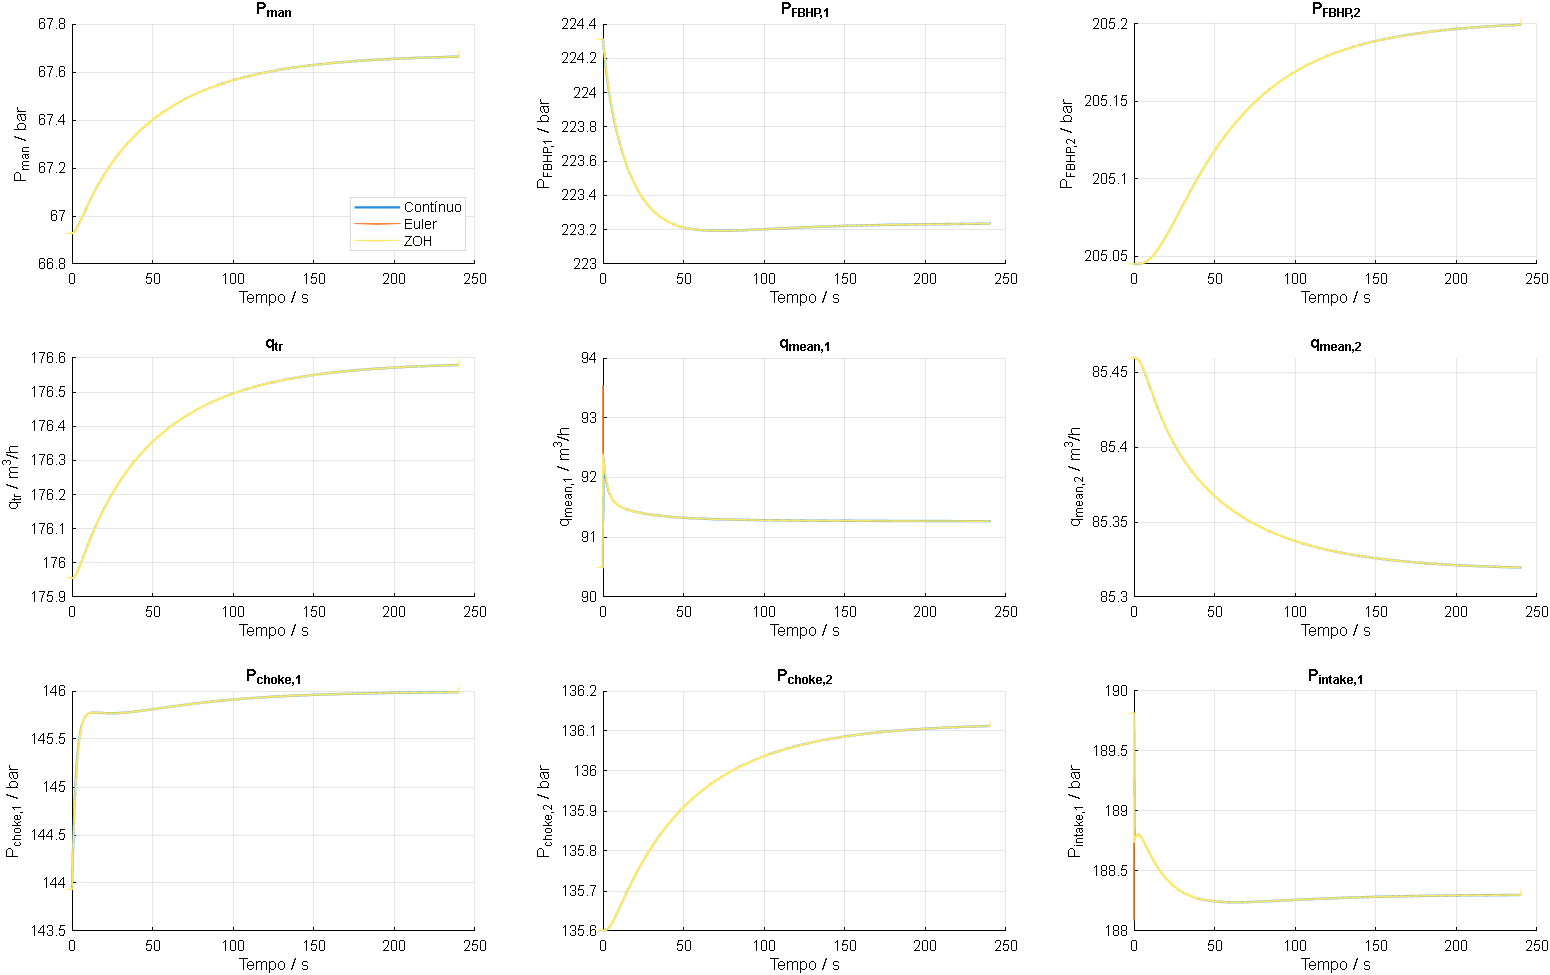
\includegraphics[width=.80\linewidth]{figuras/discretizacao.png}
\caption{Comparação entre as respostas do modelo contínuo e dos modelos discretizados por Euler e ZOH para um degrau na frequência da BCS do poço 1. Fonte: elaboração própria.}\label{fig:dis}
\end{figure}

Na Figura~\ref{fig:dis}, as respostas obtidas pelos dois métodos de discretização permanecem próximas às do modelo contínuo. O ZOH reproduz a evolução do sistema linear nos instantes de amostragem para entradas mantidas constantes, enquanto Euler fornece uma aproximação de primeira ordem, cuja precisão depende diretamente da escolha de $T_s$.

\section{Considerações finais}
A análise realizada permitiu caracterizar o comportamento dinâmico de um campo de produção de petróleo composto por dois poços operados por BCS. As simulações do modelo fenomenológico evidenciaram a interação hidráulica entre os poços e o retorno das variáveis ao regime estacionário após a retirada das perturbações. A linearização reproduziu satisfatoriamente as respostas do processo nas proximidades da condição de equilíbrio considerada.

A análise dos autovalores e das trajetórias no espaço de estados indicou estabilidade assintótica local. As formas canônicas controlável, observável e de Jordan apresentaram organizações distintas dos estados internos, preservando a relação entre a entrada e a saída selecionadas. Por fim, a discretização pelos métodos de Euler e ZOH permitiu representar a dinâmica do sistema em tempo discreto, evidenciando a influência do período de amostragem sobre a aproximação. Esses resultados constituem uma base para estudos posteriores de análise e controle do campo de produção.

\begin{thebibliography}{9}
\bibitem{ronning2011} RØNNING, R. \textit{Automatic Start-up and Control of Artificially Lifted Wells}. 2011.
\end{thebibliography}
\end{document}
